\chapter{State of play}
\graphicspath{{introduction/figures/}}

\begin{flushright}
    \small{\textit{``The true power of AI lies in its ability to augment human intelligence, not replace it.''}\\
        Andrew Ng, Co-founder of Coursera and former Chief Scientist at Baidu}
\end{flushright}

In this chapter, we embark on a journey through the landscape of existing literature and research pertinent to the convergence of open source Large Language Models (LLMs) and Retrieval-Augmented Generation (RAG) systems, in collaboration with BIGmama Technology. Our objective is to establish a robust foundation for understanding the intricacies and potentials inherent in this symbiotic relationship. As we delve into the state of play, we aim to illuminate key theoretical underpinnings and empirical insights that underpin our study of open source LLMs and Rag systems within the context of BIGmama Technology. To initiate this exploration, we contextualize our inquiry within the broader discourse of natural language processing and information retrieval, elucidating the multifaceted challenges and opportunities presented by the integration of open source LLMs and Rag systems. Subsequently, we navigate through seminal concepts and methodologies, including the principles of LLM architecture, Rag framework components, and their applications in various domains. These foundational insights serve as pillars supporting our quest to explore the potential synergies and advancements offered by the convergence of open source LLMs and Rag systems within the framework of BIGmama Technology.

\section{Presenting BIGmama Technology}

BIGmama is an innovative startup founded in France with a subsidiary in Algeria, specializing in data science and artificial intelligence solutions. With over 9 years of experience as of 2024, the company has established itself as a leading provider of bespoke predictive applications tailored to meet the unique needs of its clients.

Guided by a distinguished board of directors comprising former CEOs of global conglomerates such as Danone and Safran, BIGmama boasts a team of highly skilled data scientists and software engineers. This multidisciplinary team, consisting of more than a dozen experts in their respective fields, brings a wealth of knowledge and expertise to the company's endeavors.

BIGmama's commitment to innovation and cutting-edge technologies has allowed them to deliver state-of-the-art solutions that leverage the power of data science and artificial intelligence. With a strong focus on providing customized solutions, the company has consistently exceeded its clients' expectations, enabling them to gain valuable insights and make data-driven decisions.

Through its strategic partnerships and collaborations, BIGmama continues to push the boundaries of what is possible in the realms of data science and AI (Artificial Intelligence), positioning itself as a driving force in the ever-evolving technological landscape.

\subsection{Mission}

Beyond speeches, BIGmama's mission is to propose effective methodologies, action plans, and tools to:

\begin{itemize}
    \item Solve problems with artificial intelligence tools.
    \item Put people at the heart of technology, i.e., the hybridization of AI.
    \item Make technology a common good, shareable, and accessible to the maximum number of people who can participate and contribute.
\end{itemize}

The company's commitment extends far beyond mere rhetoric; it is dedicated to developing practical solutions, methodologies, and actionable plans to leverage the power of artificial intelligence for problem-solving. BIGmama places a strong emphasis on ensuring that technology remains human-centric, fostering a harmonious integration and hybridization of AI with human intelligence.

Moreover, BIGmama recognizes the importance of democratizing access to technology, ensuring that it becomes a shared resource that can benefit society as a whole. The company aims to create an environment where the maximum number of individuals can actively participate and contribute to the advancement of technology.

Ultimately, BIGmama's mission is to position technology as a catalyst for freedom, empowering individuals and communities to unlock new possibilities and overcome barriers through innovative solutions.

\subsection{Vision}

\begin{flushright}
    \small{\it{''Standing on the Shoulders of Giants''}}
\end{flushright}


\noindent We find ourselves at a pivotal moment in human history, where the rapid advancements in artificial intelligence are poised to reshape our world in unprecedented ways. Groundbreaking technologies like ChatGPT, developed by industry giants, are at the forefront of this transformative wave, mobilizing vast resources to redefine the boundaries of what is possible.

However, BIGmama's approach is not to compete directly with these titans but rather to harness their innovations as a springboard for its own technological endeavors. By building upon the foundations laid by these industry leaders, BIGmama aims to leverage their advancements as a catalyst for its own visionary project.

Rather than reinventing the wheel, BIGmama recognizes the value in standing on the shoulders of giants, capitalizing on their groundbreaking work to propel its own unique solutions forward. This strategic approach not only allows for more efficient progress but also fosters an environment of collaboration and synergy within the broader technological ecosystem.

With a keen understanding of the rapidly evolving landscape, BIGmama remains agile and adaptable, poised to seize opportunities presented by the advancements of industry giants. By embracing a collaborative mindset and harnessing the collective wisdom of the technological community, BIGmama is well-positioned to contribute its own innovative solutions, shaping the future in alignment with its vision and mission.

\subsection{BIGmama Specificities} \label{specificities}

One of the valuable heritages that BIGmama acquired during the 9 years of actively developing bespoke AI applications to its clients is its unique methodology of work. This methodology is centered around the following ideas :

\begin{itemize}
    \item \textbf{Data science starts with problematization:}

          At BIGmama, the approach to data science does not begin with data science itself but rather with reframing and problematization. The company's clients often arrive with a subject or topic rather than a clearly defined problem. BIGmama has developed a methodology to convert these topics into well-defined problems that data scientists can effectively tackle.

    \item \textbf{The data scientist is a "maverick":}

          BIGmama recognizes that the data scientist is a "maverick" who cannot be restrained. The company understands that it cannot impose specific tools or methods on data scientists when it comes to solving problems.

    \item \textbf{Data science a tool to solve problems:}

          BIGmama views data science not as an end in itself but as a means to solve problems. Often, the solution to their clients' problems lies outside the realm of data science tools.

    \item \textbf{Hybridization:}

          BIGmama believes that the future of AI lies in what is commonly referred to as Hybrid AI (Hybrid Artificial Intelligence). This approach encompasses a set of methodologies and techniques aimed at combining the potential of models with purely human knowledge. The company believes that this hybridization allows for putting humans at the heart of technological development and producing tools that are more efficient, easier to maintain, and less expensive.
\end{itemize}


\subsection{Products}

Historically, BIGmama is a startup specialized in the development of predictive applications for third parties. The company's approach is specific and based on the principles of hybridization between human and model capabilities. These \hyperref[specificities]{specificities} have led BIGmama to develop its own internal tools. These tools have evolved as the company's needs have changed, transitioning from \href{https://big-mama.io/en/iko}{Iko} to \href{https://www.hyko.ai}{Hyko}. BIGmama is now willing to make these tools available to the broader technology ecosystem.

As a startup with a rich history in predictive application development, BIGmama has cultivated a unique approach that emphasizes the seamless integration of human expertise and model capabilities. This distinctive methodology, rooted in the principles of hybridization, has driven the company to develop its own suite of proprietary internal tools.

Over time, as BIGmama's requirements have evolved, these tools have undergone continuous refinement and adaptation. The company has transitioned from its initial Iko platform to the more advanced Hyko solution, ensuring that its tools remain aligned with its ever-changing needs and the dynamic technological landscape.

In recognition of the value these tools hold for the broader tech community, BIGmama has made the strategic decision to make them available to the larger ecosystem. By sharing its internally developed tools, the company aims to foster collaboration, knowledge exchange, and the collective advancement of technological solutions.


\subsection{Service: Asset based consulting (ABC)}

The evolving business landscape, driven by rapid technological advancements and heightened competition, necessitates innovative solutions for optimizing operations and fostering sustainable growth. Traditional consulting approaches, such as report writing, are no longer sufficient to meet the demand for specialized solutions tailored to individual client needs. This shift has led to the emergence of asset-based consulting (ABC), a specialized field focused on creating, leveraging, and maximizing the value of a company's assets. In ABC, consultants collaborate closely with clients to identify and harness tangible and intangible assets, including technology, intellectual property, and human capital, to drive operational efficiency and gain a competitive edge. Unlike traditional consulting, ABC takes a holistic and internal perspective, recognizing the unique assets and capabilities of each organization. Consultants draw on multidisciplinary expertise to assess, diagnose, and unlock hidden value through innovative asset management strategies. As industries become increasingly complex and competitive, the demand for asset-based consulting, particularly in leveraging AI assets, continues to grow across sectors. From optimizing supply chains to capitalizing on intellectual property, asset-based consulting offers a strategic framework and expertise to help organizations achieve their objectives in a dynamic business environment.

\subsection{Hyko}

Hyko is a platform that empowers you to become an AI toolmaker. It can be thought of as using "Lego" pieces from its vast toolbox, filled with AI models (over 130,000), APIs (such as Stability.ai, OpenAI, Cohere), web scraping tools, utility functions, and more.

Hyko is a powerful platform that puts the tools and resources necessary for building AI applications at your fingertips. By offering a comprehensive toolbox and streamlined workflow, Hyko empowers users to unleash their creativity and bring their AI-powered visions to life.

\begin{figure}[!ht]
    \centering
    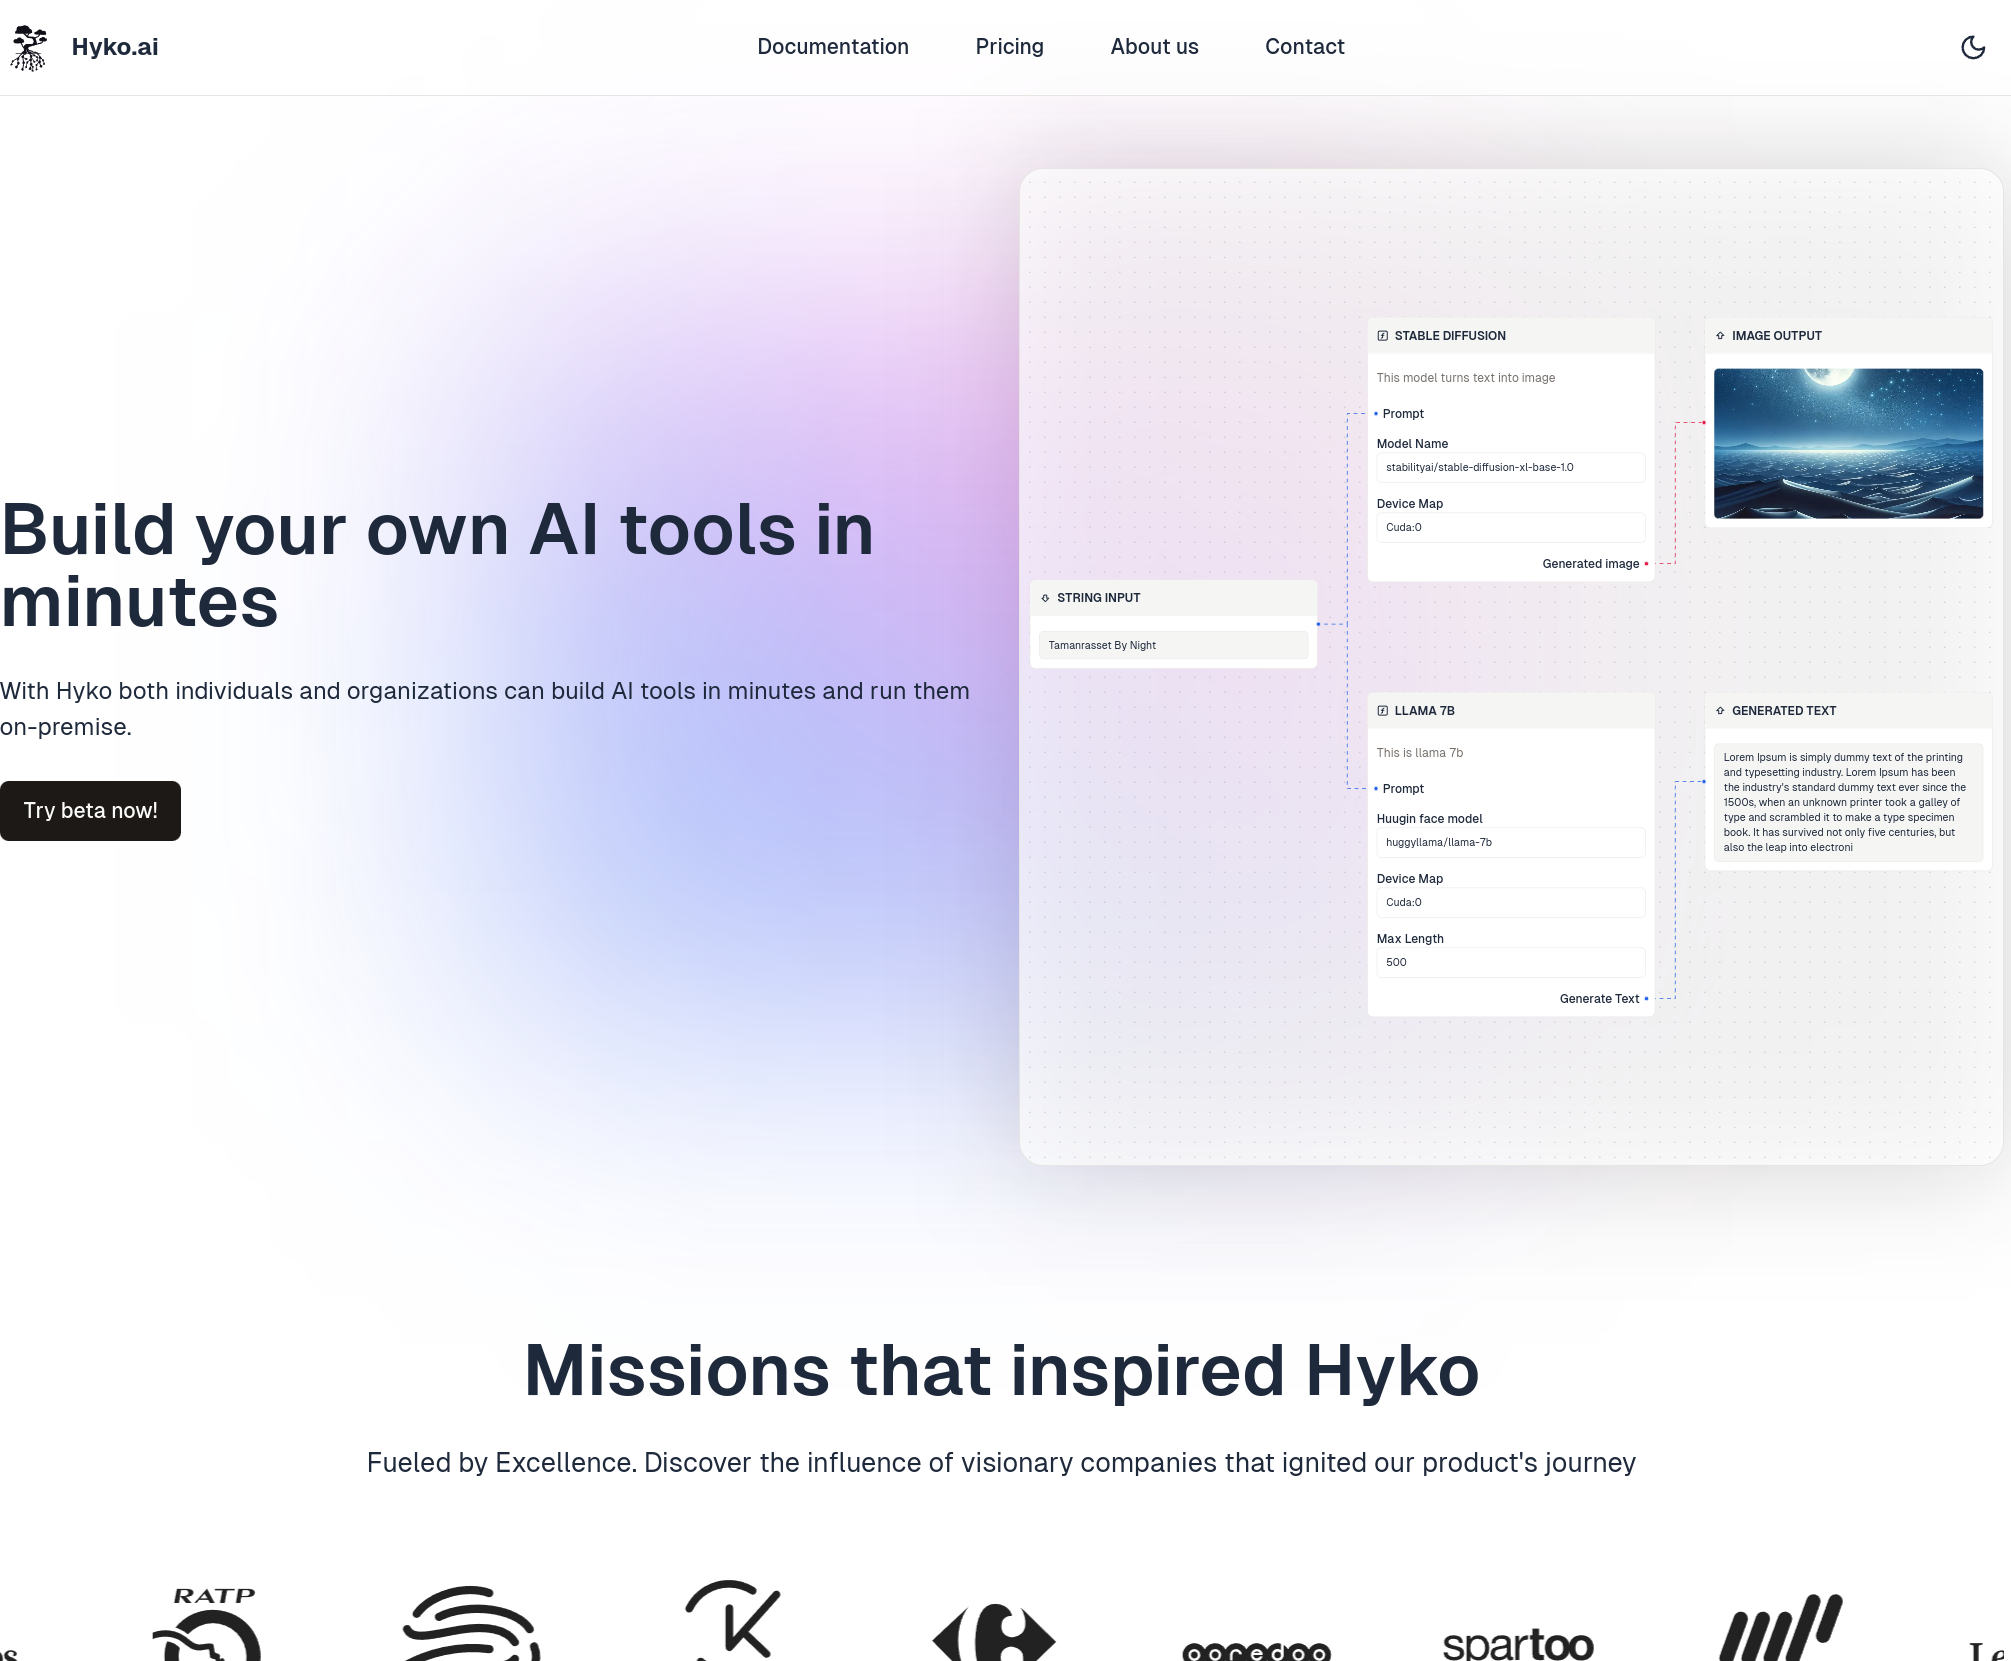
\includegraphics[width=\linewidth]{hyko.png}
    \caption{Hyko's Landing page (\url{https://www.hyko.ai})}
    \label{fig:hyko_landing_page}
\end{figure}

Many companies grapple with numerous manual tasks performed repetitively by employees, often numbering in the hundreds or thousands each month. Traditional automation tools struggled to automate these tasks fully due to their reliance on human reasoning. However, LLMs have revolutionized automation by exposing reasoning capabilities through an API.

In response to this advancement, Hyko emerged as an AI-first platform, designed not merely to streamline employee workflows but to entirely replace them from start to finish. The platform's automation builder offers unparalleled flexibility, enabling the automation of highly complex workflows with ease.

The future value of AI is anticipated to derive not solely from AI engineers or data scientists, but also from field experts who possess the capability to integrate their domain knowledge with AI technologies to address everyday challenges. This shift underscores the growing importance of domain-specific expertise in harnessing the potential of AI for practical applications.

This imperative is frequently encountered among Hyko users, who often find themselves in need of extracting vital insights from their diverse data repositories, which encompass web sources, PDF documents, and email archives. In response to this demand, Rag systems emerge as key facilitators, particularly when coupled with open-source LLMs such as Llama3, Phi3, and mixtral7B. Rag systems excel in the retrieval, aggregation, and generation of pertinent information, empowering users to distill valuable insights from their data reservoirs efficiently and effectively. This seamless integration enhances the capacity for nuanced understanding and actionable intelligence extraction, thereby augmenting the utility and versatility of Hyko across diverse information retrieval and analysis endeavors.

\section{RAG: Enhancing LLMs with External Knowledge}

LLMs showcase impressive capabilities but encounter challenges like hallucination \cite{zhang2023sirens}, outdated knowledge, and non-transparent, untraceable reasoning processes. RAG has emerged as a promising solution by incorporating knowledge from external databases. This enhances the accuracy and credibility of the generation, particularly for knowledge-intensive tasks, and allows for continuous knowledge updates and integration of domain specific information. RAG synergistically merges LLMs' intrinsic knowledge with the vast, dynamic repositories of external databases \cite{gao2024retrievalaugmented}.

General-purpose language models can be fine-tuned to achieve several common tasks such as sentiment analysis and named entity recognition. These tasks generally don't require additional background knowledge.

For more complex and knowledge-intensive tasks, it's possible to build a language model-based system that accesses external knowledge sources to complete tasks. This enables more factual consistency, improves reliability of the generated responses, and helps to mitigate the problem of "hallucination".

Meta AI researchers introduced a method called Retrieval Augmented Generation (RAG) \cite{metaairag}  to address such knowledge-intensive tasks. RAG combines an information retrieval component with a text generator model. RAG can be fine-tuned and its internal knowledge can be modified in an efficient manner and without needing retraining of the entire model.

RAG takes an input and retrieves a set of relevant/supporting documents given a source (e.g., Wikipedia). The documents are concatenated as context with the original input prompt and fed to the text generator which produces the final output. This makes RAG adaptive for situations where facts could evolve over time. This is very useful as LLMs's parametric knowledge is static. RAG allows language models to bypass retraining, enabling access to the latest information for generating reliable outputs via retrieval-based generation.

\begin{figure}[!ht]
    \centering
    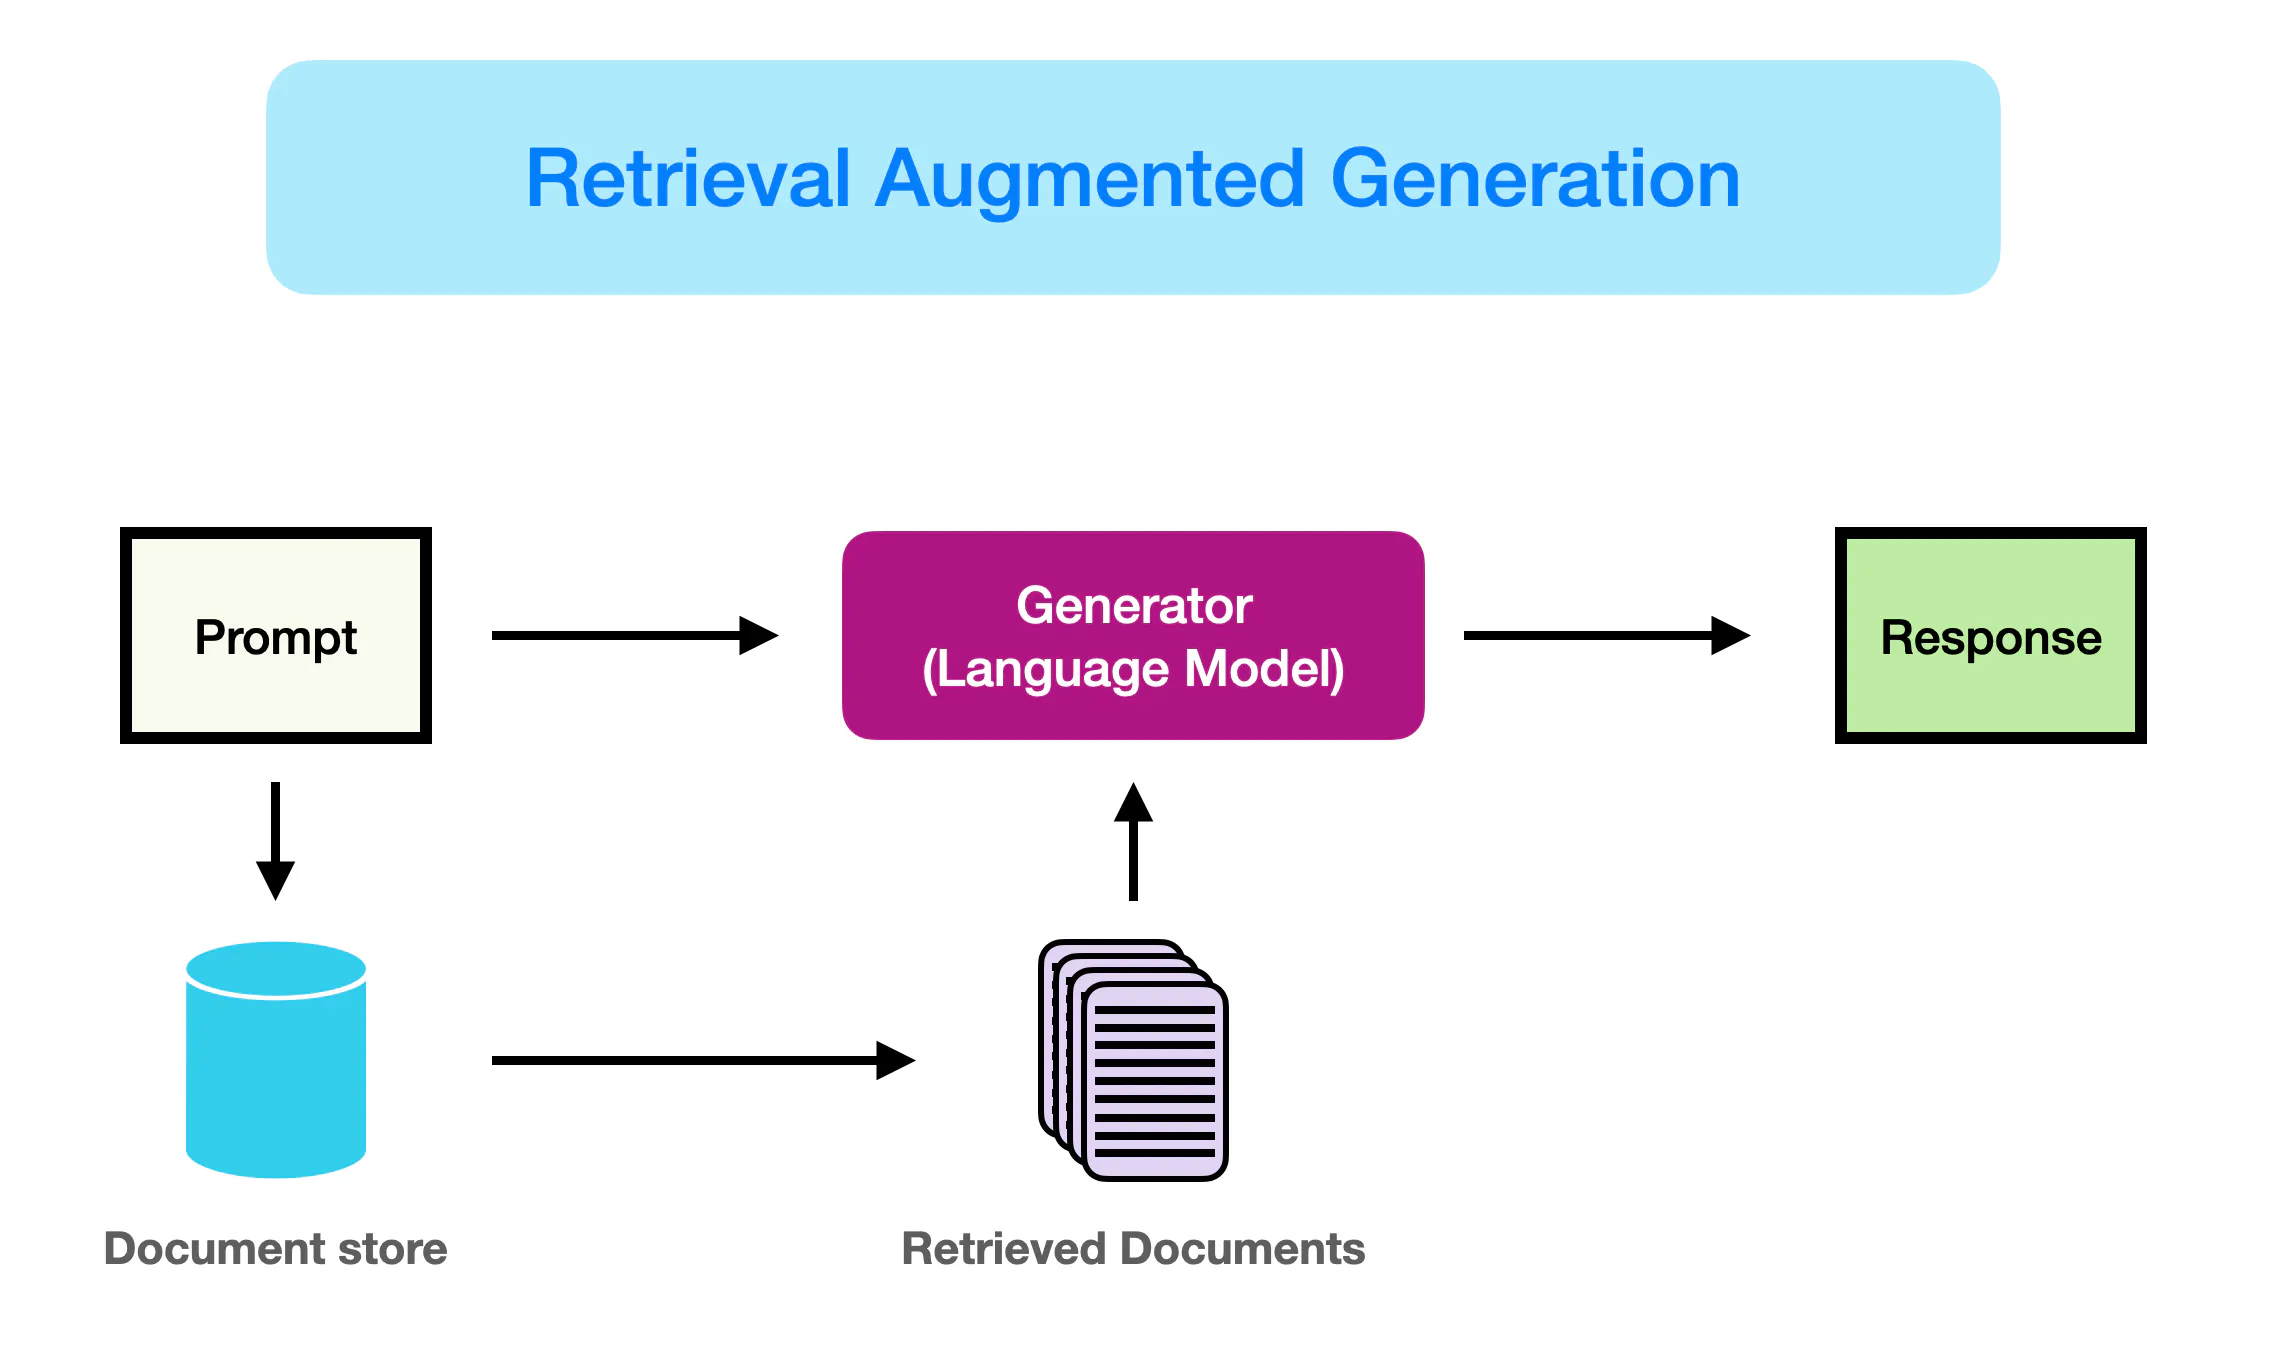
\includegraphics[width=\linewidth]{rag.png}
    \caption{Retrieval Augmented Generation. \url{https://www.promptingguide.ai/research/rag\#introduction-to-rag}}
    \label{fig:rag}
\end{figure}

In short, the retrieved evidence obtained in RAG can serve as a way to enhance the accuracy, controllability, and relevancy of the LLM's response. This is why RAG can help reduce issues of hallucination or performance when addressing problems in a highly evolving environment.

\section{Conclusion}

In this chapter, we lay the foundation for the subsequent sections of this thesis. We introduce fundamental concepts in Retrieval-Augmented Generation (RAG) systems and Large Language Models (LLMs), along with a basic overview of the host company, BIGmama Technology.